\documentclass[a4paper, 12pt]{article}

\usepackage[utf8]{inputenc}
\usepackage{amsmath}
\usepackage{indentfirst}
\usepackage{graphicx}
\usepackage{multicol,lipsum}
\usepackage{hyperref}
\usepackage{minted}

\begin{document}
%\maketitle

\begin{titlepage}
	\begin{center}
	
	%\begin{figure}[!ht]
	%\centering
	%\includegraphics[width=2cm]{c:/ufba.jpg}
	%\end{figure}

		\Huge{Instituto de Ciências Matemáticas e de Computação}\\
		\large{Departamento de Ciências de Computação}\\ 
		\large{SCC0503 - Algoritmos e Estruturas de Dados II}\\ 
		\vspace{15pt}
        \vspace{95pt}
        \textbf{\LARGE{Relatório Exercício 05}}\\
		%\title{{\large{Título}}}
		\vspace{3,5cm}
	\end{center}
	
	\begin{flushleft}
		\begin{tabbing}
			Alunos: Ryan Souza Sá Teles, Silmar Pereira da Silva Junior \\
            NUSP's: 12822062, 12623950.
			Professor: Leonardo Tórtoro Pereira\\
			%Professor co-orientador: \\
	\end{tabbing}
 \end{flushleft}
	\vspace{1cm}
	
	\begin{center}
		\vspace{\fill}
			 Junho\\
		 2022
			\end{center}
\end{titlepage}
%%%%%%%%%%%%%%%%%%%%%%%%%%%%%%%%%%%%%%%%%%%%%%%%%%%%%%%%%%%

\newpage
% % % % % % % % % % % % % % % % % % % % % % % % % %
\newpage
\tableofcontents
\thispagestyle{empty}

\newpage
\pagenumbering{arabic}
% % % % % % % % % % % % % % % % % % % % % % % % % % %
\section{Introdução}
Após o recebimento do pedido, junto aos dados da BrabaLog foi desenvolvido um codigo com o intuito de representar os dados recebidos da malha na forma de um grafo, e ultilizar de tal estrutura para encontrar o melhor ponto para ser construido um centro de distribuição, e a cidade mais periférica que é atendida pela empresa. \\
O critério para encontrar o CCD será o conceito de vertice mais central, que é o vertice de menor distância ao seu vertice mais distânte.\\
Já, a cidade mais periferica será o oposto do critério para o CCD.\\

\newpage
\section{Desenvolvimento}

O desenvolvimento do projeto fez uso das abstrações já adotadas em sala de aula e o modelo de dígrafo selecionado para trabalhar foi o de "matriz de adjâcencias".\\

[EDITAR ESSA PARTE]
**Tal decisão foi tomada pela comparação entre a complexidade das operações em comparação com a alternativa (lista de adjacências) e a frequência com que essas operações são feitas.\\
A principail operação realizada durante o algoritimo é a adição de vertices e arestas, em que a lista é O(1) em ambos, já a matriz é $O(|V|^2)$ e O(1) respectivamente. Com relação as demais ambas as abordagens tem complexidades semelhantes.\\
Outro fator que corroborou para a escolha foi a complexidade de espaço entre as opções, com a lista sendo $O(|V|+|E|)$ enquanto a matrix de adjacências sendo $O(|V|^2)$.**\\

O algoritmo de FloyWarshall já implementado em sala de aula fez uso da distância euclidiana entre os pontos (vertíces).

Para a representação do ponto cartesiano como vertíce do grafo, dentro da classe vertíce foi adotada a keyword "Record" do Java 16, que omite getters, setters e construtores quando estes fazem uso apenas dos atributos
--Citação do conteúdo https://www.guiadojava.com.br/2021/04/java-records.html

Com o objetivo de aplicar as boas práticas de código na atividade, os métodos para encontrar o vértice mais central, mais periferico, assim como o mais distante do periferico, foram implementados na classe do próprio "FloyWarshallTraversal", a qual está bem abstraida e implementada com as práticas dos padrões de projeto.\\

Abaixo, as implementações:

Implementação da classe Vertex (Representação do ponto cartesiano):

\begin{minted}[mathescape, linenos]{java}
public record Vertex(int x, int y) {

    public float euclideanDistance(Vertex other) {
        return (float) Math.sqrt(Math.pow(x - other.x, 2) + Math.pow(y - other.y, 2));
    }

    public String getName() {
        return "(" + x + "," + y + ")";
    }

    public String toString() {
        return x + "," + y;
    }
}

\end{minted}


\begin{minted}[mathescape, linenos]{java}
  
\end{minted}

Implementação da classe FloydWarshallTraversal:

\begin{minted}[mathescape, linenos]{java}

public class FloydWarshallTraversal extends TraversalStrategy {
    private static final Logger LOGGER = Logger.getLogger("FloydWarshallTraversal.class");

    public float[][] getDistanceMatrix() { return distanceMatrix;}
    public void setDistanceMatrix(float[][] distanceMatrix) {this.distanceMatrix = distanceMatrix;}

    private float[][] distanceMatrix;

    public FloydWarshallTraversal(AbstractGraph graph) {
        super(graph);
        distanceMatrix = new float[graph.getNumberOfVertices()][graph.getNumberOfVertices()];
    }

    Vertex centralVertex = null;
    Vertex peripheralVertex = null;

    @Override
    public void traverseGraph(Vertex source) {
        for (int i = 0; i < getGraph().getNumberOfVertices(); i++) {
            for (int j = 0; j < getGraph().getNumberOfVertices(); j++) {
                Vertex origin = getGraph().getVertices().get(i);
                Vertex destination = getGraph().getVertices().get(j);
                if (getGraph().edgeExists(origin, destination)) {
                    distanceMatrix[i][j] = getGraph().getDistance(origin, destination);
                } else {
                    distanceMatrix[i][j] = Float.POSITIVE_INFINITY;
                }
            }
        }
        for (int k = 0; k < getGraph().getNumberOfVertices(); k++) {
            for (int i = 0; i < getGraph().getNumberOfVertices(); i++) {
                for (int j = 0; j < getGraph().getNumberOfVertices(); j++) {
                    float newDistance = distanceMatrix[i][k] + distanceMatrix[k][j];
                    if (newDistance < distanceMatrix[i][j]) {
                        distanceMatrix[i][j] = newDistance;
                    }
                }
            }
        }
        //printDistanceMatrix();
    }

    private void printDistanceMatrix() {
        var decimalFormat = new DecimalFormat("00.00");
        var distanceMatrixString = new StringBuilder();
        distanceMatrixString.append('\n');
        for (float[] row : distanceMatrix) {
            for (float value : row) {
                distanceMatrixString.append(decimalFormat.format(value));
                distanceMatrixString.append(' ');
            }
            distanceMatrixString.append('\n');
        }
        LOGGER.info(distanceMatrixString.toString());
    }

    public Vertex getFarthestVertexFrom(Vertex source) {
        int sourceIndex = getGraph().getVertices().indexOf(source);

        int farthestVertexIndex = 0;
        float maxDistance = Float.NEGATIVE_INFINITY;
        for (int column = 0; column < distanceMatrix.length; column++) {
            if (column == sourceIndex) {
                continue;
            }
            if (maxDistance < distanceMatrix[sourceIndex][column]) {
                maxDistance = distanceMatrix[sourceIndex][column];
                farthestVertexIndex = column;
            }
        }
        return getGraph().getVertices().get(farthestVertexIndex);
    }

    public Vertex getPeripheralVertex() {
        if (peripheralVertex != null)
            return peripheralVertex;

        int peripheralVertexIndex = 0;
        float[] maximumCostVertexes = getMaximumCostInColumns();

        float max = Float.NEGATIVE_INFINITY;
        for (int i = 0; i < maximumCostVertexes.length; i++) {
            if (max < maximumCostVertexes[i]) {
                max = maximumCostVertexes[i];
                peripheralVertexIndex = i;
            }
        }

        peripheralVertex = getGraph().getVertices().get(peripheralVertexIndex);
        return peripheralVertex;
    }

    public Vertex getCentralVertex() {
        if (centralVertex != null)
            return centralVertex;

        int centralVertexIndex = 0;
        float[] maximumCostVertexes = getMaximumCostInColumns();
        float min = Float.POSITIVE_INFINITY;
        for (int i = 0; i < maximumCostVertexes.length; i++) {
            if (min > maximumCostVertexes[i]) {
                min = maximumCostVertexes[i];
                centralVertexIndex = i;
            }
        }

        centralVertex = getGraph().getVertices().get(centralVertexIndex);
        return centralVertex;
    }

    private float[] getMaximumCostInColumns() {
        float[] maximumCostVertexes = new float[distanceMatrix.length];

        for (int column = 0; column < distanceMatrix[0].length; column++) {
            float maxDistance = Float.NEGATIVE_INFINITY;
            for (int row = 0; row < distanceMatrix.length; row++) {
                if (distanceMatrix[row][column] > maxDistance) {
                    maxDistance = distanceMatrix[row][column];
                }
            }
            maximumCostVertexes[column] = maxDistance;
        }
        return maximumCostVertexes;
    }
}


\end{minted}

\newpage
\section{Resultados}
\graphicspath{ {./Results/} }

Para o caso de teste 1 temos como saída:
\begin{minted}{xml}
    INFO: Quest{
	ID: 8
	Name: Elder Care
	Description: Help the village Elder
}Quest{
	ID: 9
	Name: Second Intentions
	Description: Make the Elder tell you about the Demon Lord
}Quest{
	ID: 5
	Name: Hell's Door
	Description: You must find the entrance to the Demon Lord's Castle
}Quest{
	ID: 6
	Name: Cleaning the House
	Description: Kill all the guardians of the Demon Lord
}Quest{
	ID: 7
	Name: Showdown
	Description: Face the last fierce battle and kill the Demon Lord
}
\end{minted}

Quanto ao grafo gerado:

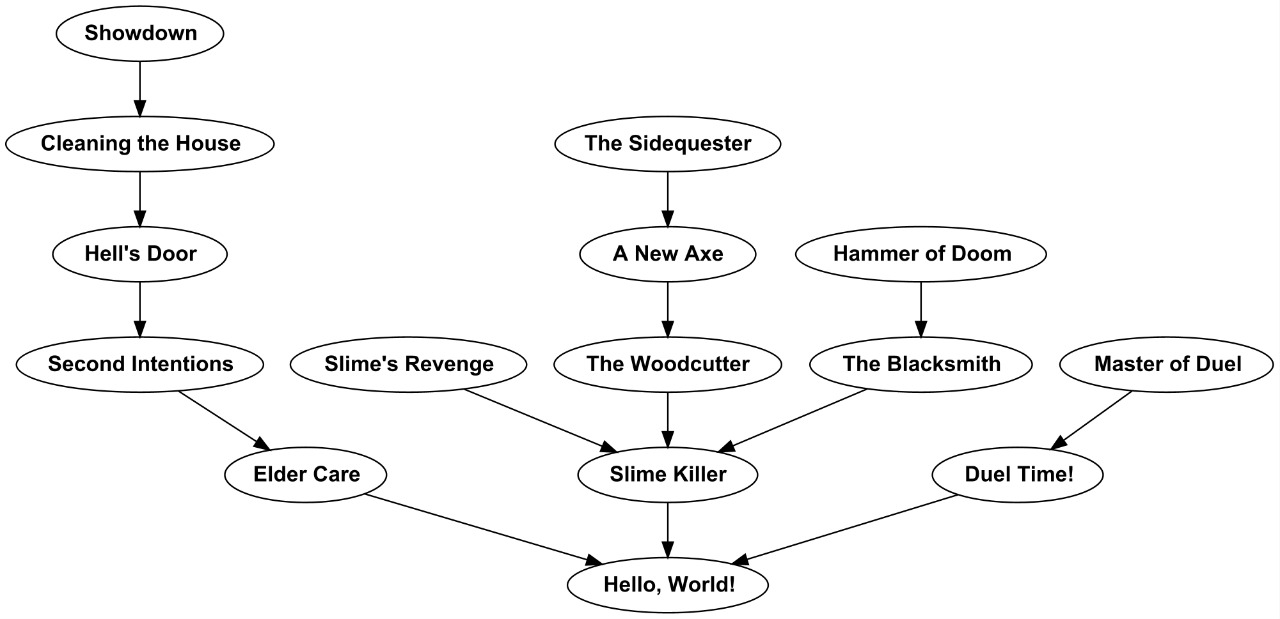
\includegraphics[width=\textwidth]{Case1.jpeg}
\\
\\

\newpage
Para o caso 2 temos como saída:

\begin{minted}{xml}
    INFO: Quest{
	ID: 0
	Name: Slime Killer
	Description: You must kill 10 slimes
}Quest{
	ID: 11
	Name: Slime's Revenge
	Description: The slime Queen wants revenge for her minions
}Quest{
	ID: 1
	Name: The Woodcutter
	Description: Find and talk to Greyson, the woodcutter
}Quest{
	ID: 2
	Name: A New Axe
	Description: Search for the legendary axe for Greyson
}Quest{
	ID: 3
	Name: The Blacksmith
	Description: Find and talk to Clint, the blacksmith
}Quest{
	ID: 4
	Name: Hammer of Doom
	Description: Search for the legendary hammer for Clint
}
\end{minted}

Quanto a seu grafo:\\

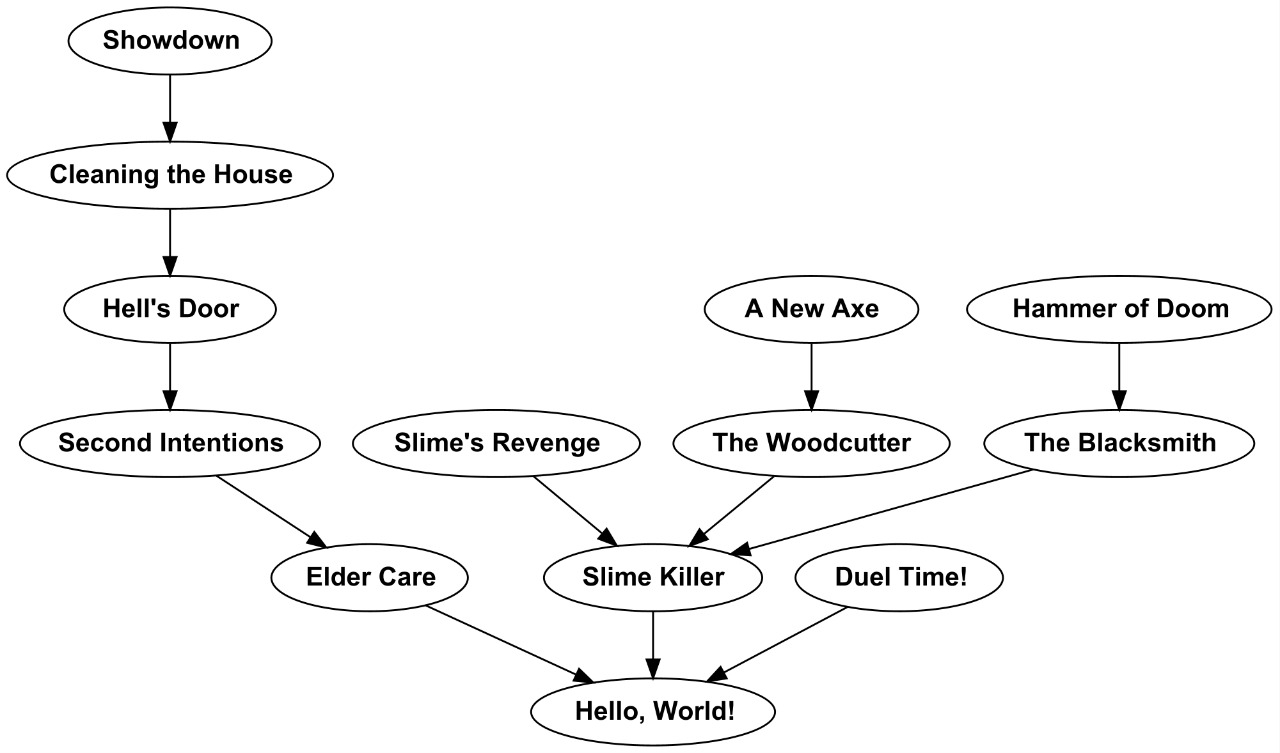
\includegraphics[width=\textwidth]{Case2.jpeg}
\\
\\

\newpage
Para o caso 3 temos como saída:


\begin{minted}{xml}
    INFO: Quest{
	ID: 10
	Name: Hello, World!
	Description: Get to the starter town and talk to the villagers
}Quest{
	ID: 0
	Name: Slime Killer
	Description: You must kill 10 slimes
}Quest{
	ID: 11
	Name: Slime's Revenge
	Description: The slime Queen wants revenge for her minions
}Quest{
	ID: 1
	Name: The Woodcutter
	Description: Find and talk to Greyson, the woodcutter
}Quest{
	ID: 2
	Name: A New Axe
	Description: Search for the legendary axe for Greyson
}Quest{
	ID: 14
	Name: The Sidequester
	Description: Face the final challenge and complete the last sidequest
}Quest{
	ID: 3
	Name: The Blacksmith
	Description: Find and talk to Clint, the blacksmith
}Quest{
	ID: 4
	Name: Hammer of Doom
	Description: Search for the legendary hammer for Clint
}Quest{
	ID: 12
	Name: Duel Time!
	Description: Win the card minigame tournament
}Quest{
	ID: 13
	Name: Master of Duel
	Description: Win the world championship card minigame tournament
}Quest{
	ID: 8
	Name: Elder Care
	Description: Help the village Elder
}Quest{
	ID: 9
	Name: Second Intentions
	Description: Make the Elder tell you about the Demon Lord
}Quest{
	ID: 5
	Name: Hell's Door
	Description: You must find the entrance to the Demon Lord's Castle
}Quest{
	ID: 6
	Name: Cleaning the House
	Description: Kill all the guardians of the Demon Lord
}Quest{
	ID: 7
	Name: Showdown
	Description: Face the last fierce battle and kill the Demon Lord
}
\end{minted}


Para seu grafo Temos:\\
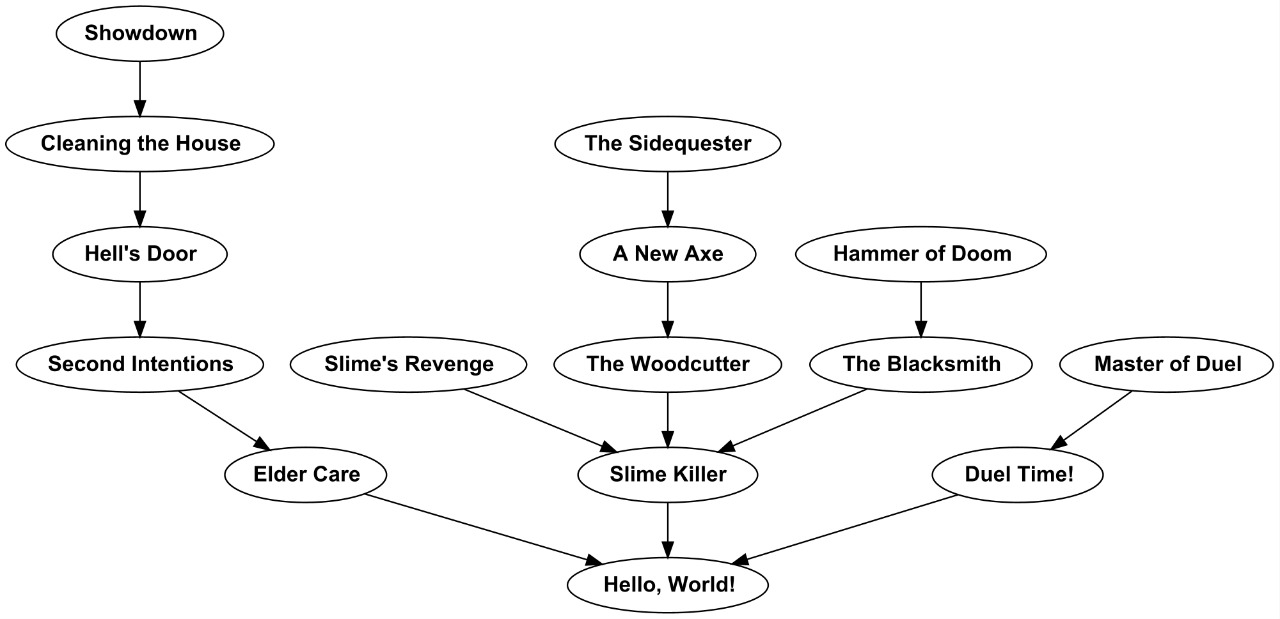
\includegraphics[width=\textwidth]{Case3.jpeg}
\\
\\


\newpage
Por fim para o caso 4 temos como saida:
\begin{minted}{xml}
    INFO: Quest{
	ID: 10
	Name: Hello, World!
	Description: Get to the starter town and talk to the villagers
}Quest{
	ID: 0
	Name: Slime Killer
	Description: You must kill 10 slimes
}Quest{
	ID: 11
	Name: Slime's Revenge
	Description: The slime Queen wants revenge for her minions
}Quest{
	ID: 1
	Name: The Woodcutter
	Description: Find and talk to Greyson, the woodcutter
}Quest{
	ID: 2
	Name: A New Axe
	Description: Search for the legendary axe for Greyson
}Quest{
	ID: 3
	Name: The Blacksmith
	Description: Find and talk to Clint, the blacksmith
}Quest{
	ID: 4
	Name: Hammer of Doom
	Description: Search for the legendary hammer for Clint
}Quest{
	ID: 12
	Name: Duel Time!
	Description: Win the card minigame tournament
}Quest{
	ID: 8
	Name: Elder Care
	Description: Help the village Elder
}Quest{
	ID: 9
	Name: Second Intentions
	Description: Make the Elder tell you about the Demon Lord
}Quest{
	ID: 5
	Name: Hell's Door
	Description: You must find the entrance to the Demon Lord's Castle
}Quest{
	ID: 6
	Name: Cleaning the House
	Description: Kill all the guardians of the Demon Lord
}Quest{
	ID: 7
	Name: Showdown
	Description: Face the last fierce battle and kill the Demon Lord
}
\end{minted}

Para seu grafo Temos:\\
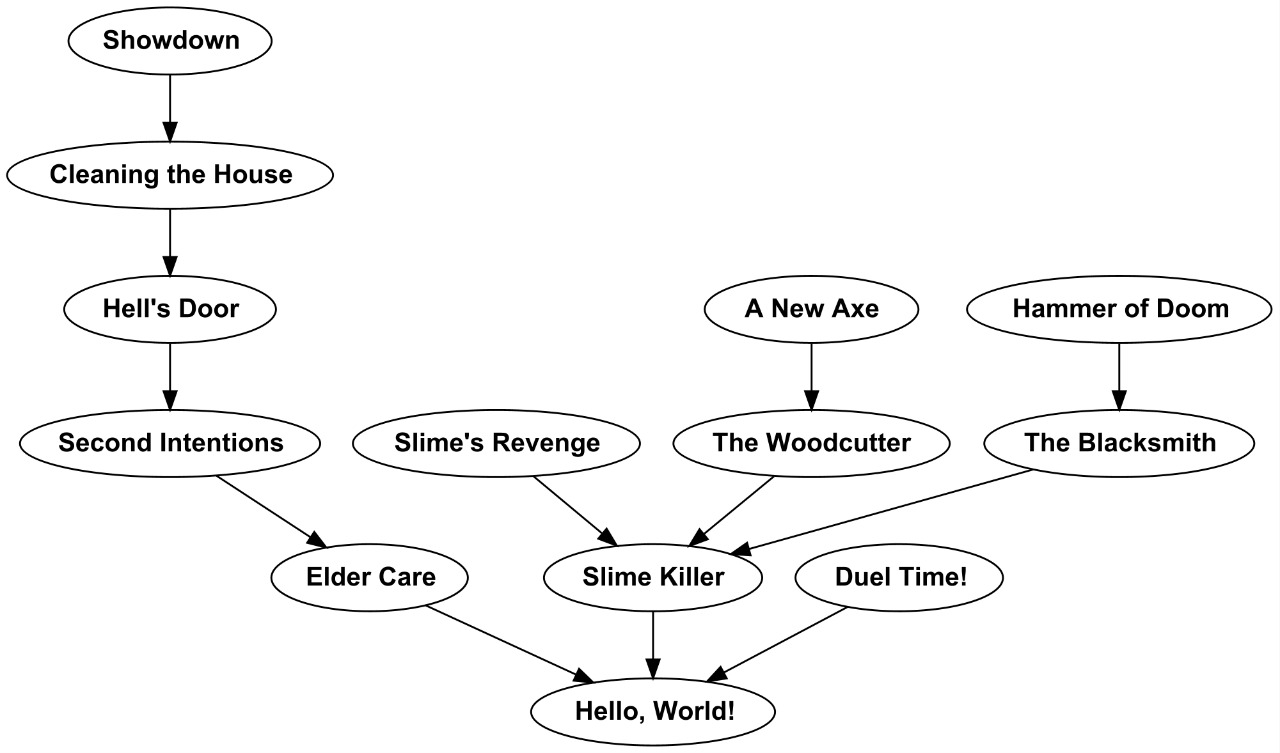
\includegraphics[width=\textwidth]{Case4.jpeg}
\\
\\
\end{document}





\newpage
\section{Resultados}
\graphicspath{ {./Results/} }


\end{document}



